\section{Results}
%
First it is important to verify that the code works correctly. This was done by comparing the results to an analytical solution and plotting the error for different problem sizes $n$. 
\begin{figure}[h!]
\begin{center}
    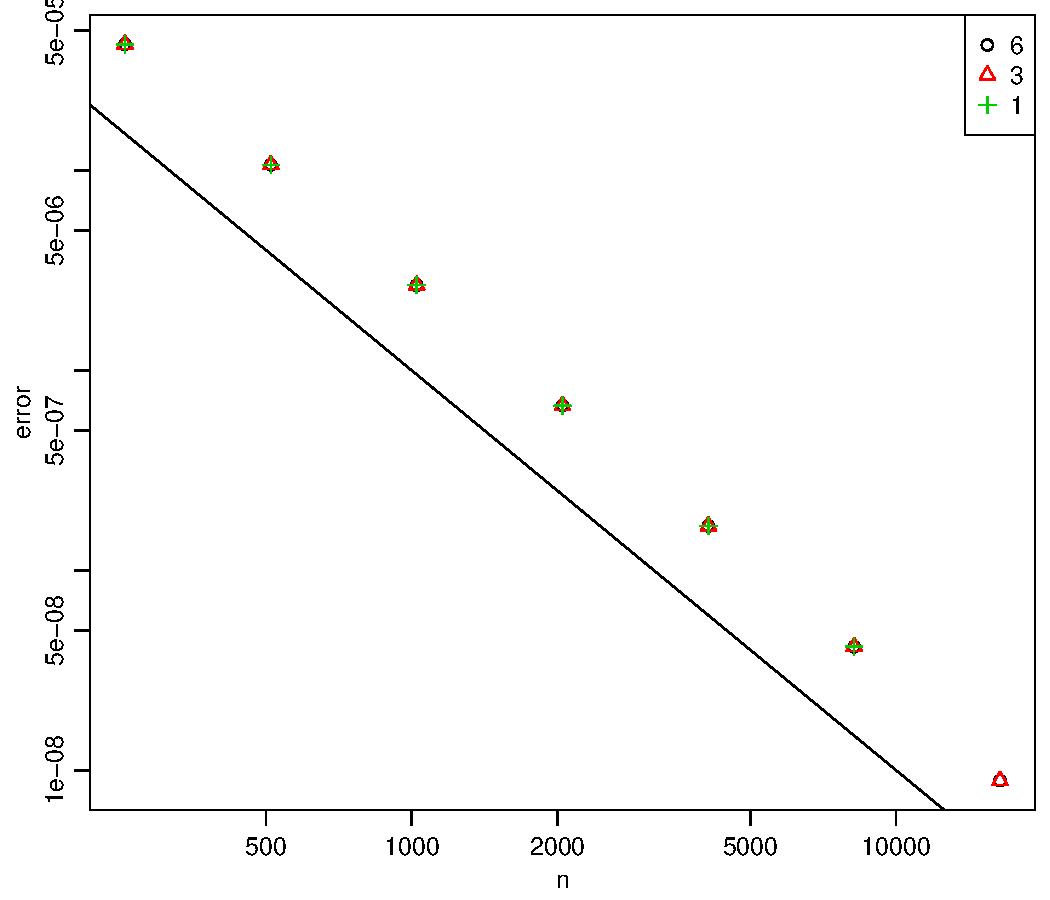
\includegraphics[scale=0.5]{./Figures/errVsn.pdf}
\end{center}
\caption{Loglog plot of the error as function of $n$. A reference line with slpe $-2$ is drawn. The problem in run on two threads with the number of processes specified in the legend.}
\label{fig:errVsn}
\end{figure}
%
Firs the problem \colorbox{yellow}{what problem?} was run on a single node where all 12 processors were utilized. The point was to investigate the performance of using threads versus MPI processes. Thus the relation between threads $t$ and processes $p$ is $p t = 12$ or $p = 12/t$. The calculations were done with $n = 2^{14}$. 
The same problem was repeated on three nodes where all 12 processors were utilized in the same way as above. The results can be found in Figure~\ref{fig:taskc}. It is clear from both plots that it is preferable to use only MPI processes and no openMP. 

While running only one MPI process and 12 threads on one node there is still some overhead from the MPI sending to itself and the work of reordering the data. Therefore the problem was solved on 12 threads without this overhead. The results are the red crosses in Figure~\ref{fig:taskc}. It is clear that it is a lot faster than with the MPI sending, but it is still slower than running with 12 MPI processes. 
\begin{figure}[h!]
  \centering
  \begin{subfigure}[b]{0.48\textwidth}
    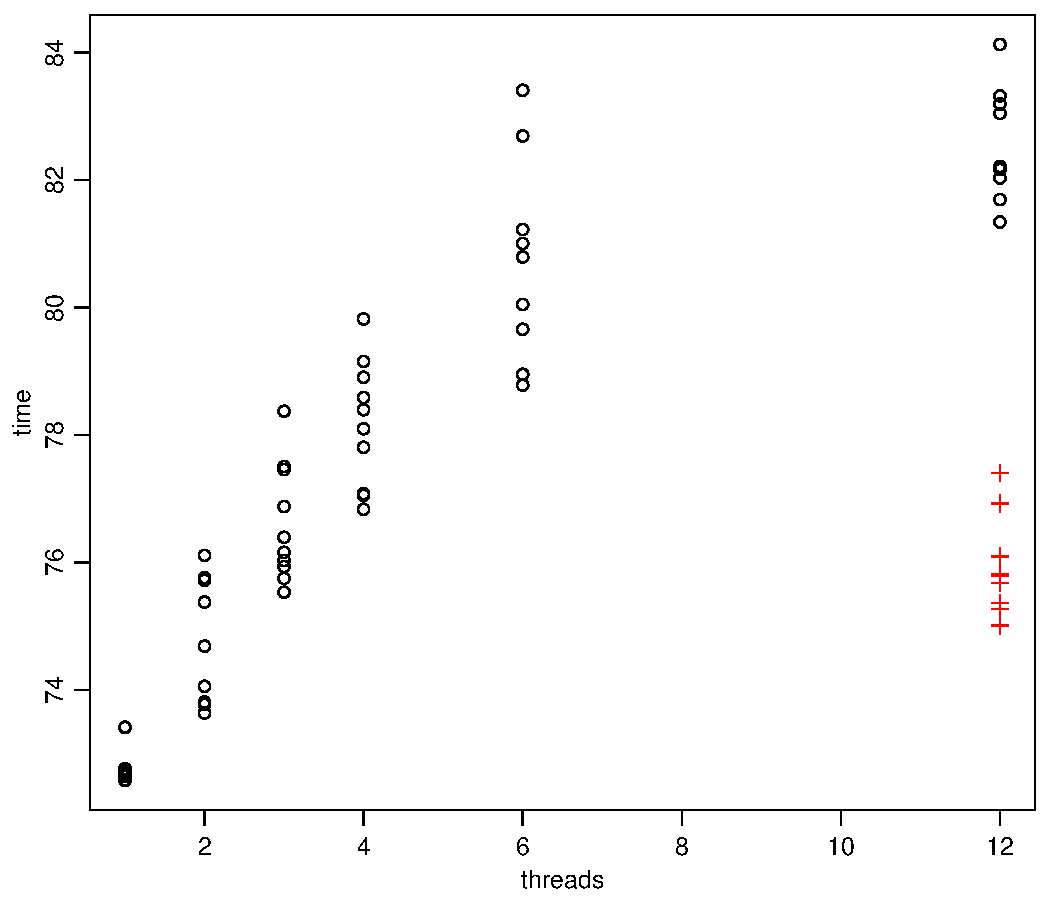
\includegraphics[width=\textwidth]{./Figures/taskc1.pdf}
  \end{subfigure}%
  \quad
  \begin{subfigure}[b]{0.48\textwidth}
    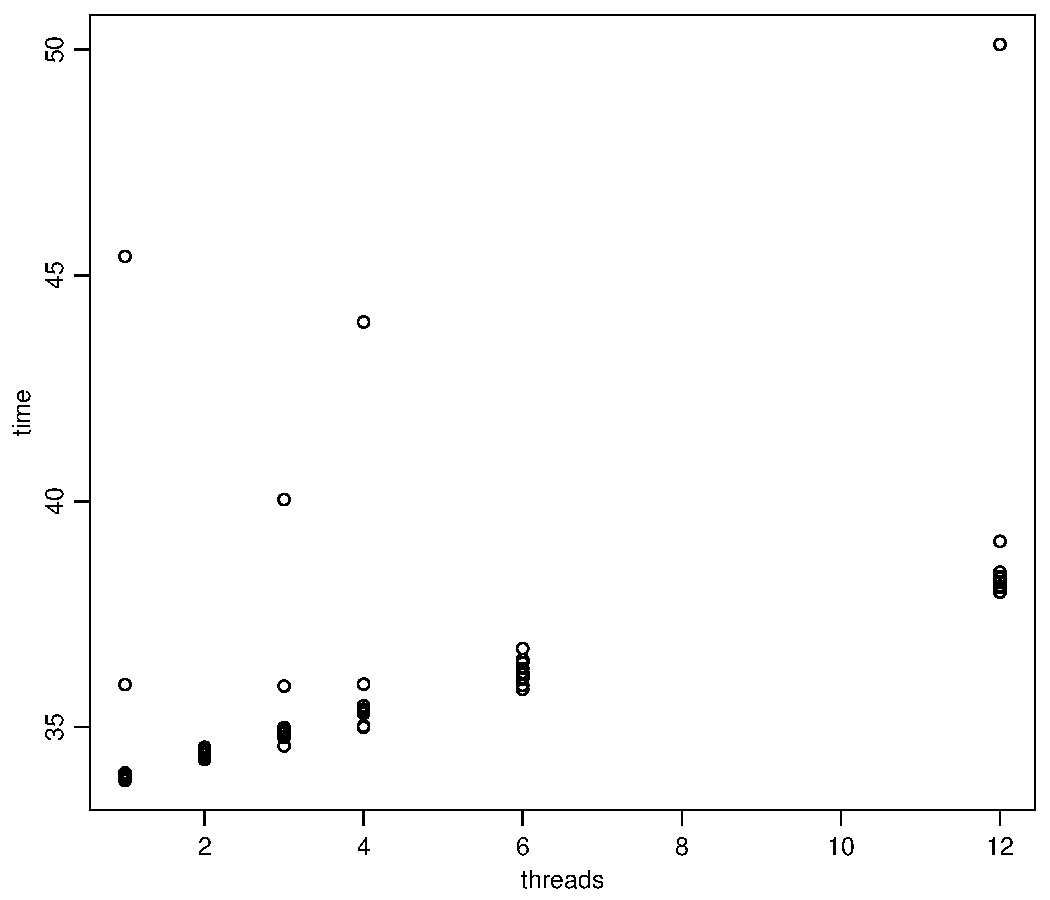
\includegraphics[width=\textwidth]{./Figures/taskc2.pdf}
  \end{subfigure}
          %(or a blank line to force the subfigure onto a new line)
  \vspace{1\baselineskip}
  \caption{Times (in seconds) for running MPI processes vs threads with $n = 2^{14}$. The total number of processors used are 12 per node, so the number of processes per node is 12 - threads. The left figure is run on one node, while the right is run on three nodes. The red crosses are run without any MPI sending at all.}
  \label{fig:taskc}
\end{figure}
%
%
\begin{figure}[h!]
  \centering
  \begin{subfigure}[b]{0.48\textwidth}
    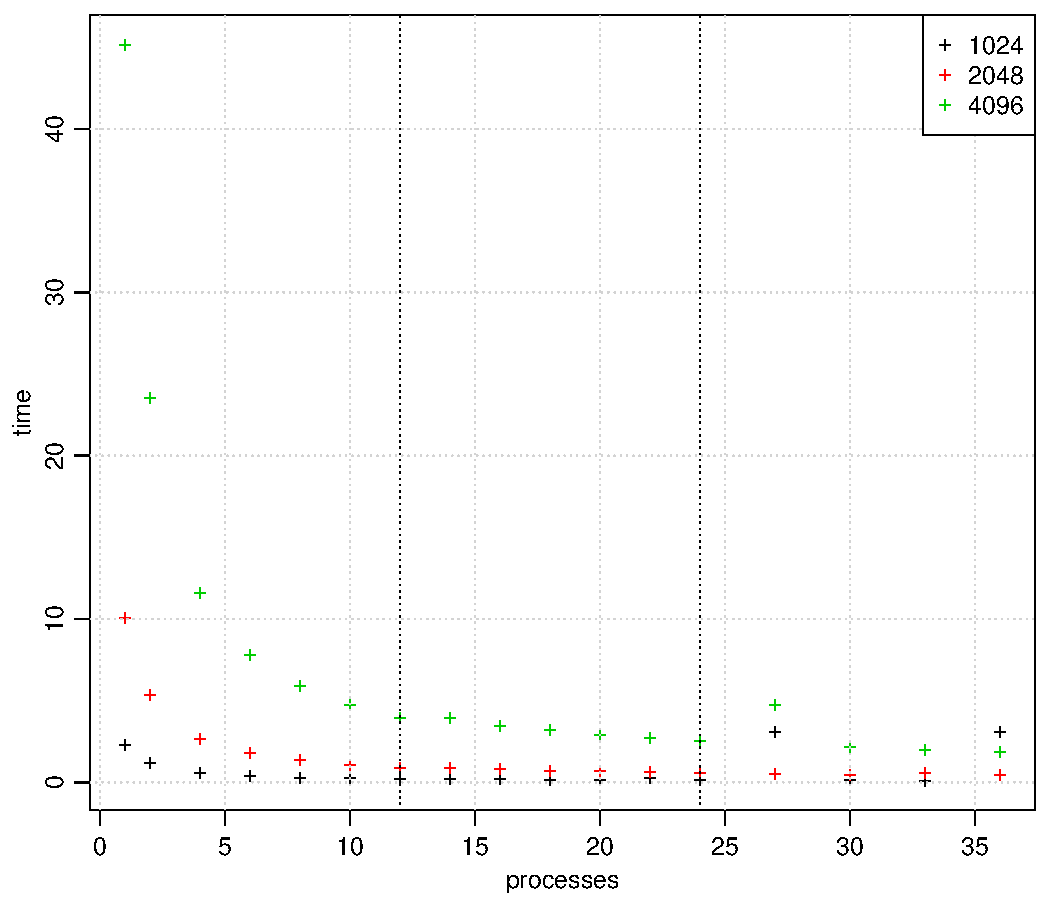
\includegraphics[width=\textwidth]{./Figures/taskbTimeProc1.pdf}
  \end{subfigure}%
  \quad
  \begin{subfigure}[b]{0.48\textwidth}
    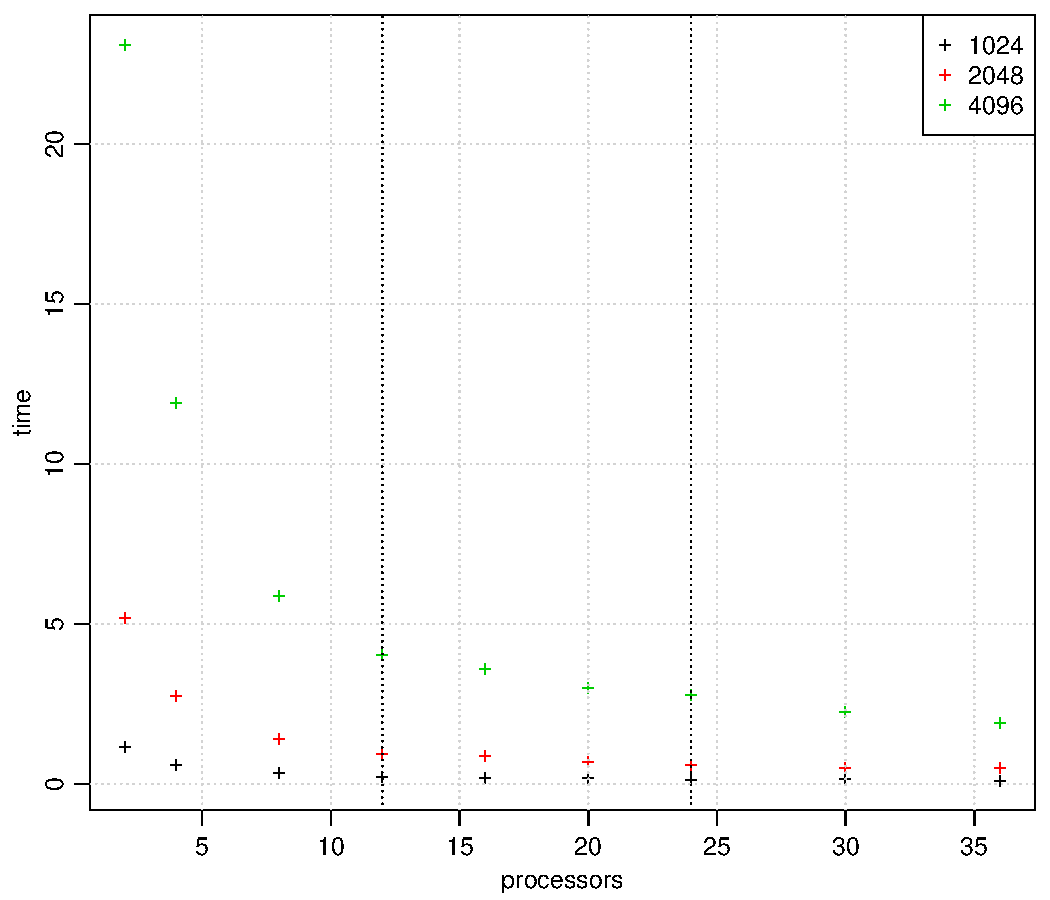
\includegraphics[width=\textwidth]{./Figures/taskbTimeProc2.pdf}
  \end{subfigure}
  \quad
  \begin{subfigure}[b]{0.48\textwidth}
    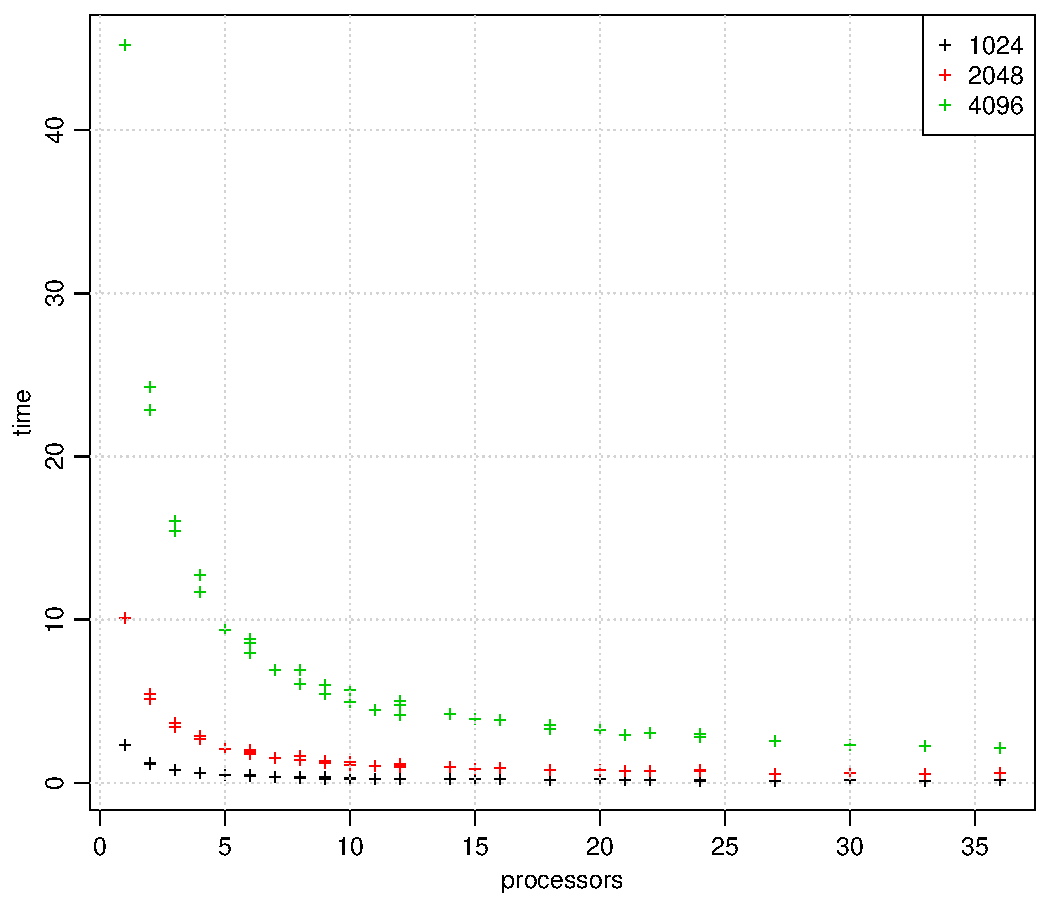
\includegraphics[width=\textwidth]{./Figures/taskbTimeNodesTimesThreads.pdf}
  \end{subfigure}
          %(or a blank line to force the subfigure onto a new line)
  \vspace{1\baselineskip}
  \caption{Times for running problem with different amount of processes. In the upper left figure each process has one thread, while in the upper right, each process has two treads. The problem is run on as few nodes as possible, and the processes are identically distributed among the nodes. The problem size $n$ is specified in the plots. In the bottom figure only one MPI process is run per node. Between 1 and 12 threads are run on each node.}
  \label{fig:time}
\end{figure}
%
\begin{figure}[h!]
  \centering
  \begin{subfigure}[b]{0.48\textwidth}
    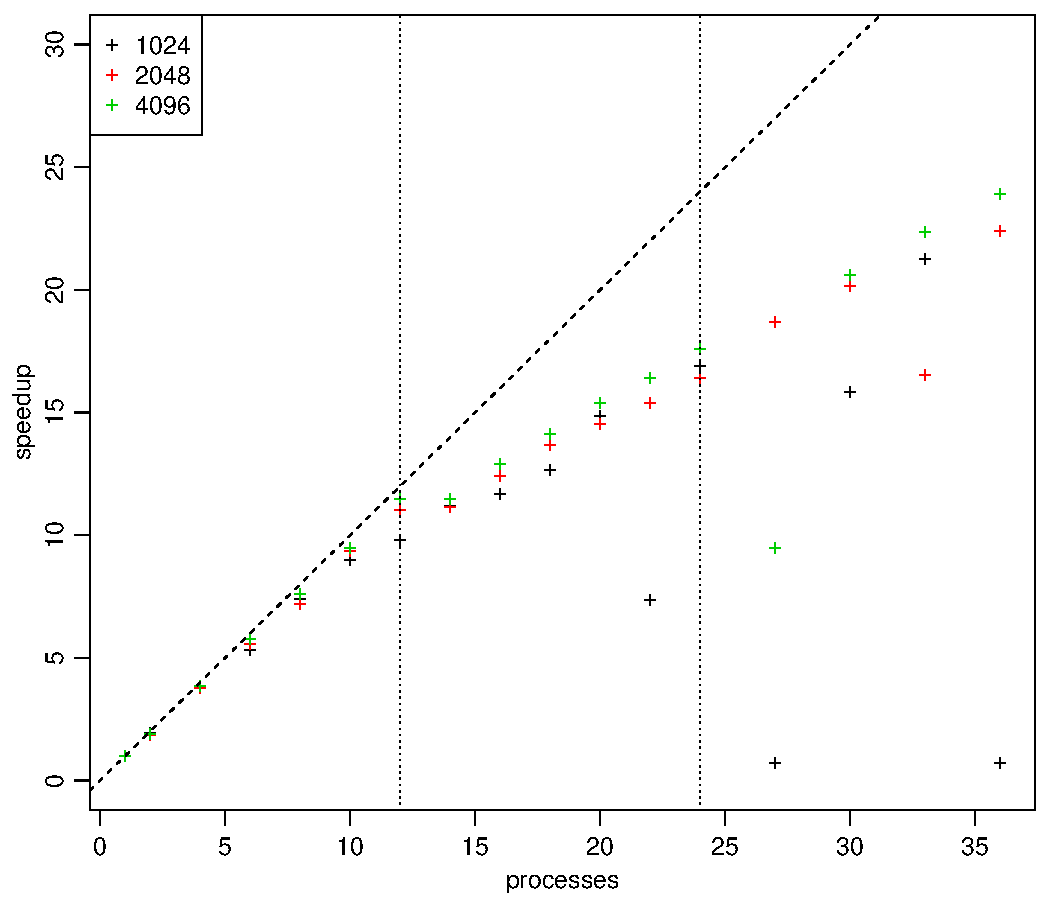
\includegraphics[width=\textwidth]{./Figures/taskbSpeedupProc1.pdf}
  \end{subfigure}%
  \quad
  \begin{subfigure}[b]{0.48\textwidth}
    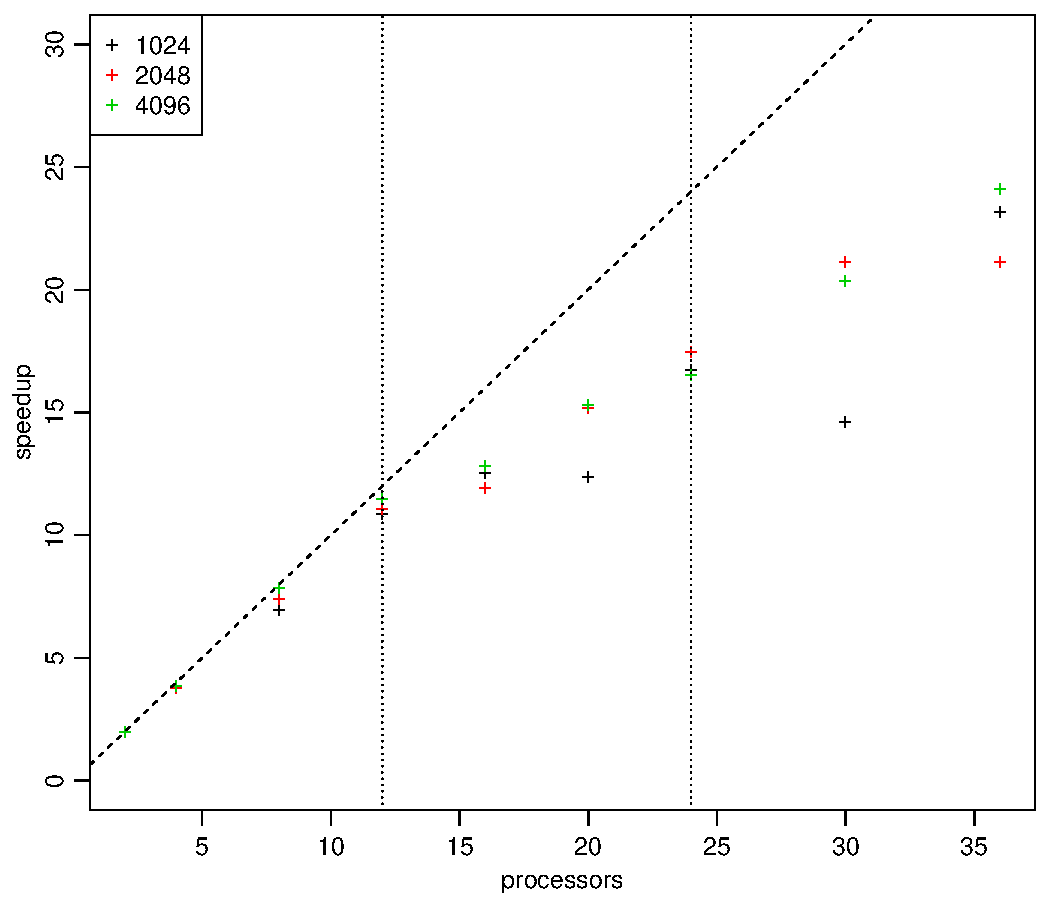
\includegraphics[width=\textwidth]{./Figures/taskbSpeedupProc2.pdf}
  \end{subfigure}
  \quad
  \begin{subfigure}[b]{0.48\textwidth}
    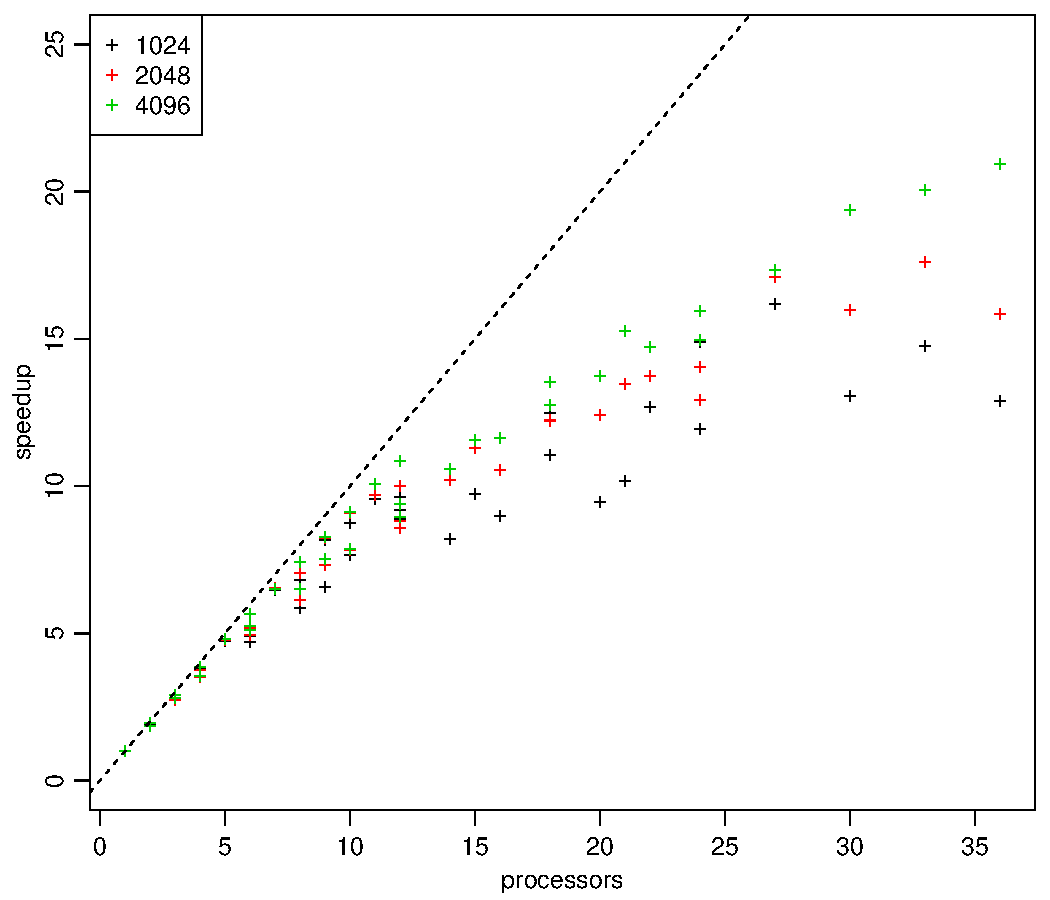
\includegraphics[width=\textwidth]{./Figures/taskbSpeedupNodesTimesThreads.pdf}
  \end{subfigure}
          %(or a blank line to force the subfigure onto a new line)
  \vspace{1\baselineskip}
  \caption{Speedup for running problem with different amount of processes. In the upper left figure each process has one thread, while in the upper right, each process has two treads. The problem is run on as few nodes as possible, and the processes are identically distributed among the nodes. There are drawn vertical lines to show when a new node is utilized, and a line with slope 1. The problem size $n$ is specified in the plots. In the bottom figure only one MPI process is run per node. Between 1 and 12 threads are run on each node.}
  \label{fig:Speedup}
\end{figure}
%
\begin{figure}[h!]
  \centering
  \begin{subfigure}[b]{0.48\textwidth}
    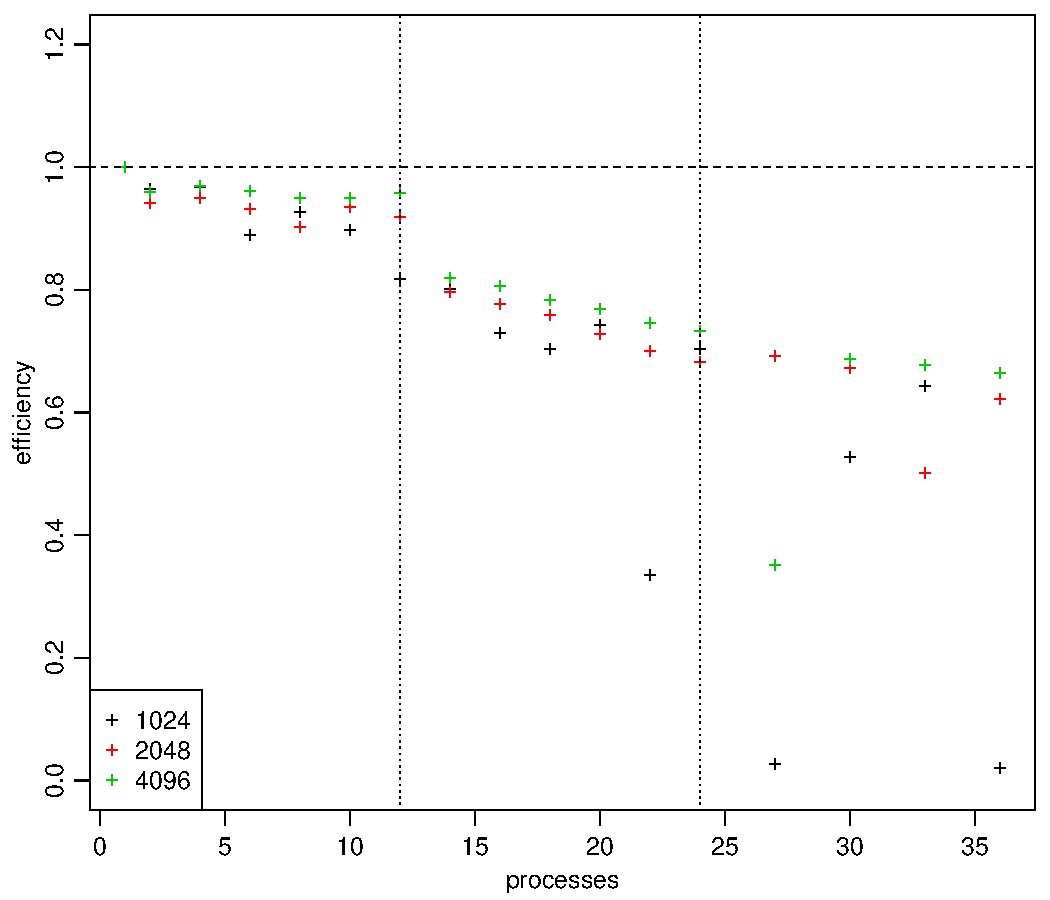
\includegraphics[width=\textwidth]{./Figures/taskbEfficiencyProc1.pdf}
  \end{subfigure}%
  \quad
  \begin{subfigure}[b]{0.48\textwidth}
    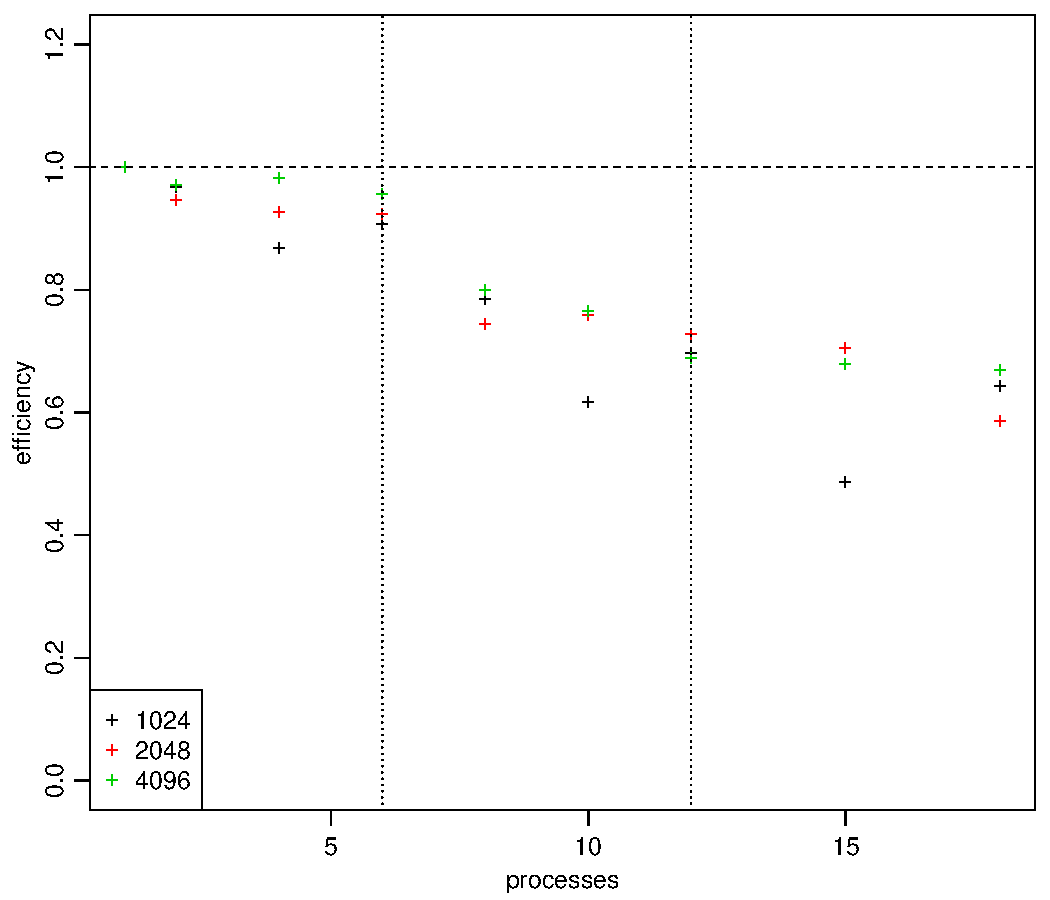
\includegraphics[width=\textwidth]{./Figures/taskbEfficiencyProc2.pdf}
  \end{subfigure}
          %(or a blank line to force the subfigure onto a new line)
  \vspace{1\baselineskip}
  \caption{Efficiency for running problem with different amount of processes. In the upper left figure each process has one thread, while in the upper right, each process has two treads. The problem is run on as few nodes as possible, and the processes are identically distributed among the nodes. There are drawn vertical lines to show when a new node is utilized, and a horizontal line at 1. The problem size $n$ is specified in the plots. In the bottom figure only one MPI process is run per node. Between 1 and 12 threads are run on each node.}
  \label{fig:Efficiency}
\end{figure}
%
\begin{figure}[h!]
\begin{center}
    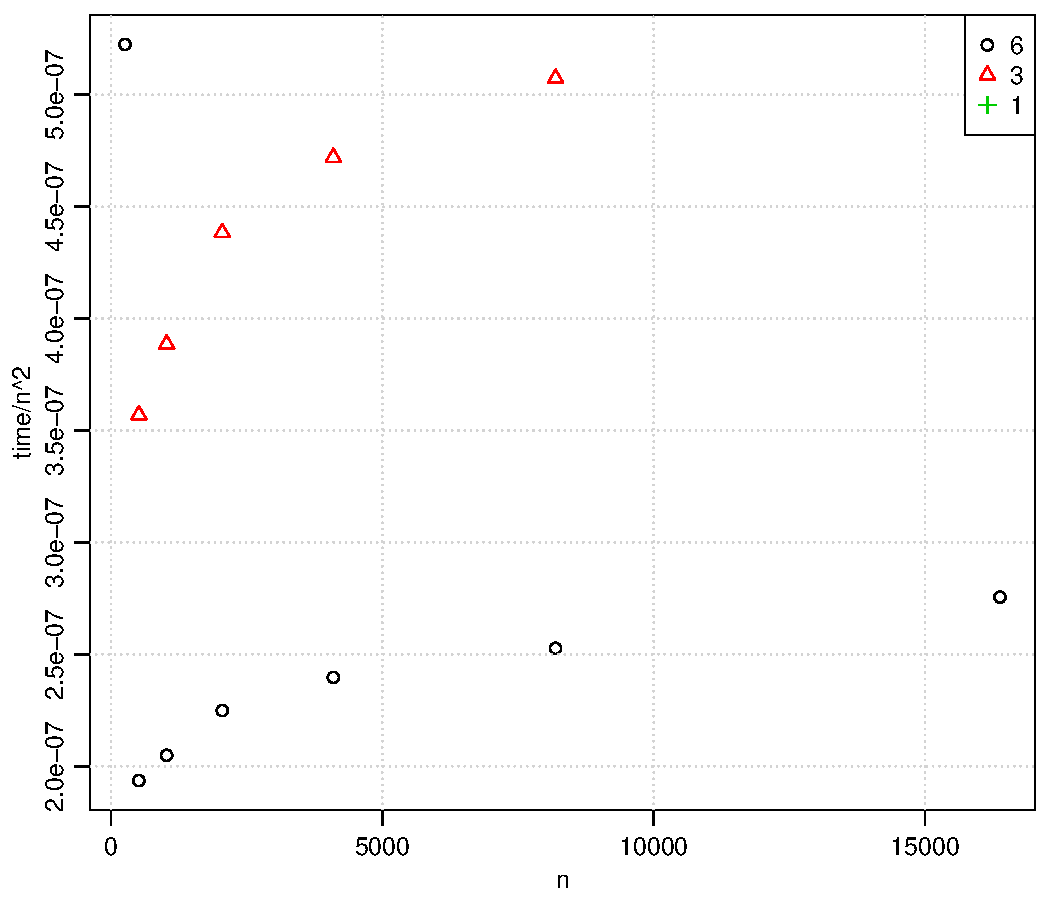
\includegraphics[scale=0.5]{./Figures/timeOverN2Vsn.pdf}
\end{center}
\caption{$Time/n^2$ as function of $n$. Illustrates how time scales with $n^2$. The data is the same as in Figure~\ref{fig:errVsn}}
\label{fig:timeOverN2Vsn}
\end{figure}

